\documentclass[aspectratio=169]{beamer}\usepackage[]{graphicx}\usepackage[]{color}
% maxwidth is the original width if it is less than linewidth
% otherwise use linewidth (to make sure the graphics do not exceed the margin)
\makeatletter
\def\maxwidth{ %
  \ifdim\Gin@nat@width>\linewidth
    \linewidth
  \else
    \Gin@nat@width
  \fi
}
\makeatother

\definecolor{fgcolor}{rgb}{0.345, 0.345, 0.345}
\newcommand{\hlnum}[1]{\textcolor[rgb]{0.686,0.059,0.569}{#1}}%
\newcommand{\hlstr}[1]{\textcolor[rgb]{0.192,0.494,0.8}{#1}}%
\newcommand{\hlcom}[1]{\textcolor[rgb]{0.678,0.584,0.686}{\textit{#1}}}%
\newcommand{\hlopt}[1]{\textcolor[rgb]{0,0,0}{#1}}%
\newcommand{\hlstd}[1]{\textcolor[rgb]{0.345,0.345,0.345}{#1}}%
\newcommand{\hlkwa}[1]{\textcolor[rgb]{0.161,0.373,0.58}{\textbf{#1}}}%
\newcommand{\hlkwb}[1]{\textcolor[rgb]{0.69,0.353,0.396}{#1}}%
\newcommand{\hlkwc}[1]{\textcolor[rgb]{0.333,0.667,0.333}{#1}}%
\newcommand{\hlkwd}[1]{\textcolor[rgb]{0.737,0.353,0.396}{\textbf{#1}}}%
\let\hlipl\hlkwb

\usepackage{framed}
\makeatletter
\newenvironment{kframe}{%
 \def\at@end@of@kframe{}%
 \ifinner\ifhmode%
  \def\at@end@of@kframe{\end{minipage}}%
  \begin{minipage}{\columnwidth}%
 \fi\fi%
 \def\FrameCommand##1{\hskip\@totalleftmargin \hskip-\fboxsep
 \colorbox{shadecolor}{##1}\hskip-\fboxsep
     % There is no \\@totalrightmargin, so:
     \hskip-\linewidth \hskip-\@totalleftmargin \hskip\columnwidth}%
 \MakeFramed {\advance\hsize-\width
   \@totalleftmargin\z@ \linewidth\hsize
   \@setminipage}}%
 {\par\unskip\endMakeFramed%
 \at@end@of@kframe}
\makeatother

\definecolor{shadecolor}{rgb}{.97, .97, .97}
\definecolor{messagecolor}{rgb}{0, 0, 0}
\definecolor{warningcolor}{rgb}{1, 0, 1}
\definecolor{errorcolor}{rgb}{1, 0, 0}
\newenvironment{knitrout}{}{} % an empty environment to be redefined in TeX

\usepackage{alltt}
\usepackage{multirow}
%\usecolortheme{beaver}
%\usecolortheme[RGB={129,3,3}]{structure}
\usetheme{CambridgeUS}
\usecolortheme{seahorse}

% Standard header (will need to change date!)
\title[GEOG 5680 Summer '20]{GEOG 5680\\Introduction to R}
\subtitle[Intro]{12: Spatial data in R}
\author[S. Brewer]{Simon Brewer}
\institute[Univ. Utah]{
  Geography Department\\
  University of Utah\\
  Salt Lake City, Utah 84112\\[1ex]
  \texttt{simon.brewer@geog.utah.edu}
}
\date[May 06, 2020]{May 06, 2020}
\IfFileExists{upquote.sty}{\usepackage{upquote}}{}
\begin{document}


%--- the titlepage frame -------------------------%
\begin{frame}
  \titlepage
\end{frame}

% \section{Objectives}
% %--- Slide 3 ----------------%
% \begin{frame}{Objectives}
% \begin{itemize}
%   \item Spatial data in R
%   \item Vector data (points, lines, polygons)
%   \item Raster data
% \end{itemize}
% \end{frame}
% 
\section{Spatial data in R}
%--- Slide ----------------%
\begin{frame}[fragile]{Spatial data in R}
From Cressie (1991):
\begin{itemize}
  \item	Point processes (occurrences of events in space)
	\item	Areal or lattice --- discrete variation of values aggregated across regular or irregular regions
	\item	Geostatistical --- continuous variation of values
\end{itemize}
Expressed as geometric features: 
\begin{itemize}
	\item Points/Lines/Areal units (polygons)/Regular grids
	\item In a plane, or, less frequently, on a surface
\end{itemize}

\end{frame}

%--- Slide ----------------%
\begin{frame}{Spatial data in R}
Packages in R dealing with spatial data (from Bivand et al)
\begin{center}
	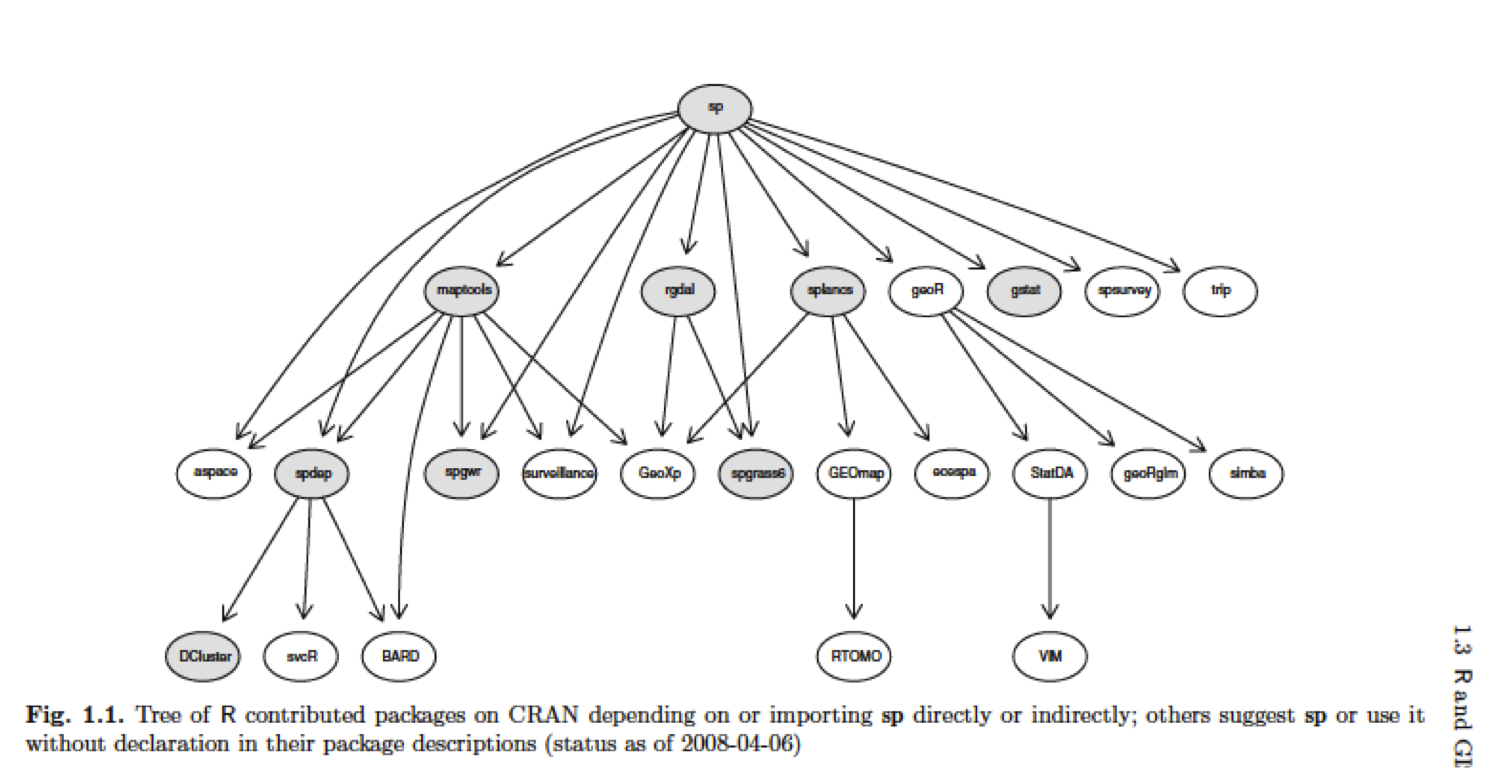
\includegraphics[width=0.9\textwidth]{./images/spatialdataclasses.png}
\end{center}
\end{frame}

%--- Slide ----------------%
\begin{frame}{Spatial data in R}
Key spatial packages:
\begin{itemize}
	\item \textbf{sp} provides the class information to deal with spatial data
	\item \textbf{raster} --- raster data and analysis
	\item \textbf{rgdal}: GDAL API interface for import/export
	\item \textbf{rgeos}: spatial geometry operations
	\item \textbf{maptools} provides many functions for read and transforming data
\end{itemize}
Most other spatial analysis packages depend on these!
\begin{itemize}
	\item \textbf{spatstat} --- analysis of spatial point processes
	\item \textbf{spatdep} --- spatial dependency
	\item \textbf{spatialreg} --- spatial regression models
	\item \textbf{gstat} --- geostatistical analysis
\end{itemize}
\end{frame}

\subsection{Spatial* data classes}
%--- Slide ----------------%
\begin{frame}{Spatial data classes in \textbf{sp}}
\begin{tabular}{|l|l|}
	\hline
	Class & Data type \\
	\hline
	SpatialPoints & Point locations \\
	SpatialPointsDataFrame & Point locations with values\\
	SpatialPolygons & Polygon vertices \\
	SpatialPolygonsDataFrame & Polygons with values\\
	SpatialGrid & Grid or raster \\
	SpatialGridDataFrame & Grid/raster with values\\
	SpatialPixel & Grid stored as point data  \\
	SpatialPixelDataFrame & Point grid with values\\
	\hline
\end{tabular}
\\Note also \texttt{ppp} (point process objects) in \textbf{spatstat} package
\end{frame}

%--- Slide ----------------%
\begin{frame}{Spatial data classes in \textbf{sp}}
Each Spatial* object has a series of \emph{slots} which contain both data and metadata about the object:
\begin{itemize}
	\item Coordinates
	\item Bounding box
	\item Coordinate Reference System
	\item Grid topology
	\item Data
	  \begin{itemize}
	    \item This is a data frame and can be acessed with indices, conditional selection, \texttt{subset()}
	  \end{itemize}
	\item Etc$\ldots$
\end{itemize}
\end{frame}

%--- Slide ----------------%
\begin{frame}[fragile]{Spatial data classes in \textbf{sp}}
\begin{knitrout}\scriptsize
\definecolor{shadecolor}{rgb}{0.969, 0.969, 0.969}\color{fgcolor}\begin{kframe}
\begin{alltt}
\hlstd{oregon} \hlkwb{=} \hlkwd{readOGR}\hlstd{(}\hlstr{"oregon/orotl.shp"}\hlstd{)}
\end{alltt}
\begin{verbatim}
## OGR data source with driver: ESRI Shapefile 
## Source: "/Users/u0784726/Dropbox/DB Docs/Classes/GEOG5680/Modules/12 Spatial data in R/oregon/orotl.shp", layer: "orotl"
## with 36 features
## It has 1 fields
\end{verbatim}
\begin{alltt}
\hlkwd{slotNames}\hlstd{(oregon)}
\end{alltt}
\begin{verbatim}
## [1] "data"        "polygons"    "plotOrder"   "bbox"        "proj4string"
\end{verbatim}
\begin{alltt}
\hlkwd{slot}\hlstd{(oregon,}\hlstr{"data"}\hlstd{)}
\end{alltt}
\begin{verbatim}
##          NAME
## 0     Clatsop
## 1    Columbia
## 2    Umatilla
## 3     Wallowa
## 4      Morrow
## 5       Union
## 6     Gilliam
## 7   Tillamook
## 8  Washington
## 9     Sherman
## 10  Multnomah
## 11 Hood River
## 12      Wasco
## 13  Clackamas
## 14    Yamhill
## 15     Marion
## 16      Baker
## 17       Polk
## 18    Wheeler
## 19    Lincoln
## 20      Grant
## 21  Jefferson
## 22       Linn
## 23     Benton
## 24      Crook
## 25    Malheur
## 26  Deschutes
## 27       Lane
## 28     Harney
## 29    Douglas
## 30    Klamath
## 31       Lake
## 32       Coos
## 33    Jackson
## 34      Curry
## 35  Josephine
\end{verbatim}
\end{kframe}
\end{knitrout}
\end{frame}

%--- Slide ----------------%
\begin{frame}[fragile]{Spatial data classes in \textbf{sp}}
\begin{knitrout}\scriptsize
\definecolor{shadecolor}{rgb}{0.969, 0.969, 0.969}\color{fgcolor}\begin{kframe}
\begin{alltt}
\hlkwd{names}\hlstd{(oregon)}
\end{alltt}
\begin{verbatim}
## [1] "NAME"
\end{verbatim}
\begin{alltt}
\hlstd{oregon}\hlopt{$}\hlstd{NAME}
\end{alltt}
\begin{verbatim}
##  [1] "Clatsop"    "Columbia"   "Umatilla"   "Wallowa"    "Morrow"    
##  [6] "Union"      "Gilliam"    "Tillamook"  "Washington" "Sherman"   
## [11] "Multnomah"  "Hood River" "Wasco"      "Clackamas"  "Yamhill"   
## [16] "Marion"     "Baker"      "Polk"       "Wheeler"    "Lincoln"   
## [21] "Grant"      "Jefferson"  "Linn"       "Benton"     "Crook"     
## [26] "Malheur"    "Deschutes"  "Lane"       "Harney"     "Douglas"   
## [31] "Klamath"    "Lake"       "Coos"       "Jackson"    "Curry"     
## [36] "Josephine"
\end{verbatim}
\begin{alltt}
\hlkwd{subset}\hlstd{(oregon, NAME}\hlopt{==}\hlstr{"Columbia"}\hlstd{)}
\end{alltt}
\begin{verbatim}
## An object of class "SpatialPolygonsDataFrame"
## Slot "data":
##       NAME
## 1 Columbia
## 
## Slot "polygons":
## [[1]]
## An object of class "Polygons"
## Slot "Polygons":
## [[1]]
## An object of class "Polygon"
## Slot "labpt":
## [1] -123.08754   45.93831
## 
## Slot "area":
## [1] 0.2103192
## 
## Slot "hole":
## [1] FALSE
## 
## Slot "ringDir":
## [1] 1
## 
## Slot "coords":
##            [,1]     [,2]
##  [1,] -122.9282 45.71420
##  [2,] -122.9289 45.72883
##  [3,] -122.9949 45.72867
##  [4,] -122.9941 45.74154
##  [5,] -123.0327 45.74257
##  [6,] -123.0334 45.77141
##  [7,] -123.3597 45.77115
##  [8,] -123.3623 46.14432
##  [9,] -123.3035 46.14491
## [10,] -123.2476 46.14419
## [11,] -123.2112 46.17017
## [12,] -123.1750 46.18375
## [13,] -123.1173 46.17948
## [14,] -123.0494 46.15590
## [15,] -122.9729 46.11065
## [16,] -122.8985 46.07949
## [17,] -122.8742 46.02735
## [18,] -122.8065 45.94405
## [19,] -122.8050 45.90424
## [20,] -122.7829 45.86805
## [21,] -122.7833 45.85061
## [22,] -122.7868 45.80051
## [23,] -122.7631 45.76073
## [24,] -122.7713 45.72785
## [25,] -122.7966 45.72540
## [26,] -122.7970 45.71529
## [27,] -122.9282 45.71420
## 
## 
## 
## Slot "plotOrder":
## [1] 1
## 
## Slot "labpt":
## [1] -123.08754   45.93831
## 
## Slot "ID":
## [1] "1"
## 
## Slot "area":
## [1] 0.2103192
## 
## 
## 
## Slot "plotOrder":
## [1] 1
## 
## Slot "bbox":
##         min        max
## x -123.3623 -122.76308
## y   45.7142   46.18375
## 
## Slot "proj4string":
## CRS arguments: NA
\end{verbatim}
\end{kframe}
\end{knitrout}
\end{frame}

% %--- Slide ----------------%
% \begin{frame}[fragile]{Map projections}
% <<echo=FALSE>>=
% orotl <- readShapeSpatial("oregon/orotl.shp")
% ortann <- readShapeSpatial("oregon/oregontann.shp")
% @
% \begin{itemize}
% 	\item The library \textbf{sp} has a function to provide projection information for Spatial* objects
% 	\item Requires a `proj4string': a list of parameters relevant to the projection
% 	\item Set projection to Lon/Lat
% \end{itemize}
% <<echo=TRUE>>=
% slot(oregon,"proj4string")
% proj4string(oregon) = CRS("+proj=longlat +ellps=WGS84")
% slot(oregon,"proj4string")
% @
% \end{frame}
% 
% %--- Slide ----------------%
% \begin{frame}[fragile]{Map projections}
% \begin{itemize}
% 	\item More complex example (Albers Equal Area), uses the \texttt{spTransform()} function to reproject (from the \textbf{rgdal} library)
% 	\item Based on PROJ.4 library
% \end{itemize}
% <<echo=TRUE, tidy=FALSE>>=
% slot(oregon,"proj4string")
% aea.proj <- "+proj=aea +lat_1=29.5 +lat_2=45.5 +lat_0=37.5 +lon_0=-110 
% 	+x_0=0 +y_0=0 +ellps=GRS80 +datum=NAD83 +units=m"
% oregon.proj <- spTransform(oregon, CRS(aea.proj))
% slot(oregon.proj,"proj4string")
% @
% <<echo=FALSE, tidy=FALSE>>=
% proj4string(ortann) = CRS("+proj=longlat +ellps=WGS84")
% ortann.proj <- spTransform(ortann, CRS(aea.proj))
% @
% \end{frame}
% 
% %--- Slide ----------------%
% \begin{frame}[fragile]{Map projections}
% \begin{columns}
% 	\begin{column}{0.5\textwidth}
% <<echo=FALSE>>=
% plot(oregon, main="Long/Lat projection", axes=T)
% plot(ortann, add=TRUE, pch=16)
% @
% 	\end{column}
% 	\begin{column}{0.5\textwidth}
% <<echo=FALSE>>=
% plot(oregon.proj, main="Albers equal area projection", axes=T)
% plot(ortann.proj, add=TRUE, pch=16)
% @
% 	\end{column}
% \end{columns}
% \end{frame}
% 
% %--- Slide ----------------%
% \begin{frame}[fragile]{Visualizing spatial data}
% \begin{columns}
% 	\begin{column}{0.5\textwidth}
% 		\begin{itemize}
% 			\item \textbf{sp} package provides function \texttt{spplot()}, which will provide basic plots of most Spatial* objects
% 			\item More flexibility can be obtained by using plot() functions
% 		\end{itemize}
% 	\end{column}
% 	\begin{column}{0.5\textwidth}
% <<echo=FALSE>>=
% NY8 = readShapePoly("./NY_data/NY8_utm18.shp")
% @
% <<echo=FALSE, cache=FALSE>>=
% spplot(NY8,"POP8")
% @
% 	\end{column}
% \end{columns}
% \end{frame}
% 
% %--- Slide ----------------%
% \begin{frame}[fragile]{Visualizing spatial data}
% \begin{columns}
% 	\begin{column}{0.5\textwidth}
% 		\begin{itemize}
% 			\item Uses two packages \textbf{classInt} and \textbf{RColorBrewer}
% 			\item \textbf{classInt} uses a data set to define intervals for color classes (quantiles, fixed, etc)
% 			\item \textbf{RColorBrewer} provides color scales for maps	
% 		\end{itemize}
% 	\end{column}
% 	\begin{column}{0.5\textwidth}
% <<echo=FALSE>>=
% display.brewer.all()
% @
% 	\end{column}
% \end{columns}
% \end{frame}
% 
% %--- Slide ----------------%
% \begin{frame}[fragile]{Visualizing spatial data}
% \begin{columns}
% 	\begin{column}{0.5\textwidth}
% <<echo=FALSE>>=
% ppt <- read.csv("swiss_ppt.csv")
% swiss.sp <- SpatialPointsDataFrame(cbind(ppt$x, ppt$y),data.frame(ppt=ppt$ppt,elev=ppt$elev))
% swiss.bord <- readShapeSpatial("borders/borders.shp")
% 
% nclr = 8
% plotvar <- swiss.sp$ppt
% class <- classIntervals(plotvar, nclr, style = "quantile",
% dataPrecision = 2)
% plotclr <- brewer.pal(nclr, "GnBu")
% colcode <- findColours(class, plotclr, digits = 3)
% 
% plot(swiss.sp, col = colcode, pch=16, axes = T)
% plot(swiss.sp, pch=1, add=T)
% plot(swiss.bord, add=T)
% title(main = "Swiss Precipitation Data")
% legend("topleft", legend = names(attr(colcode, "table")), fill = attr(colcode, "palette"), cex = 0.8)
% @
% 	\end{column}
% 	\begin{column}{0.5\textwidth}
% <<echo=FALSE>>=
% swiss.dem <- read.asciigrid("swiss_dem.grd",colname='elev')
% swiss.dem <- as(swiss.dem,'SpatialPixelsDataFrame')
% nclr <- 9
% plotvar <- swiss.dem$elev
% class <- classIntervals(plotvar, nclr, style = "quantile", dataPrecision = 2)
% plotclr <- rev(brewer.pal(nclr, "YlGn"))
% colcode <- findColours(class, plotclr, digits = 3)
% image(swiss.dem, col=plotclr, axes=T, breaks=class$brks)
% title(main = "Swiss 1km DEM")
% legend("topleft", legend = names(attr(colcode,"table")), 
%   fill = attr(colcode, "palette"), cex=0.8)
% @
% 	\end{column}
% \end{columns}
% \end{frame}
% 
% %--- Slide ----------------%
% \begin{frame}{Data import/export}
% \begin{itemize}
% 	\item \textbf{maptools} package
% 	\item Allows import and export of shapefiles
% 	\item \texttt{readShapeSpatial()} and \texttt{writeSpatialShape()}
% 	\item Also \texttt{readShapePoly()}, \texttt{readShapeLines()}, etc
% 	\item NB --- work best with Spatial*DataFrame objects
% 	\item Also has tools for converting to/from classes
% \end{itemize}
% \end{frame}
% 
% % %--- Slide ----------------%
% % \begin{frame}{Data import/export}
% % \begin{itemize}
% % 	\item \textbf{rgdal} package (uses GDAL/OGR library)
% % 	\item Allows import and export of most raster formats (ArcInfo/GeoTIFF/ESRI/Most RS images)
% % 	\item See also \texttt{readAsciiGrid()} in \textbf{maptools} (reads ESRI grids)
% % 	\item \textbf{raster} package (large files), \textbf{ncdf} package, \textbf{shapefile} package
% % 
% % \end{itemize}
% % \end{frame}
% % 
% %--- Slide ----------------%
% \begin{frame}{Writing to kml files}
% \texttt{kmlPoints()} function in \textbf{maptools} package:
% \begin{center}
% 	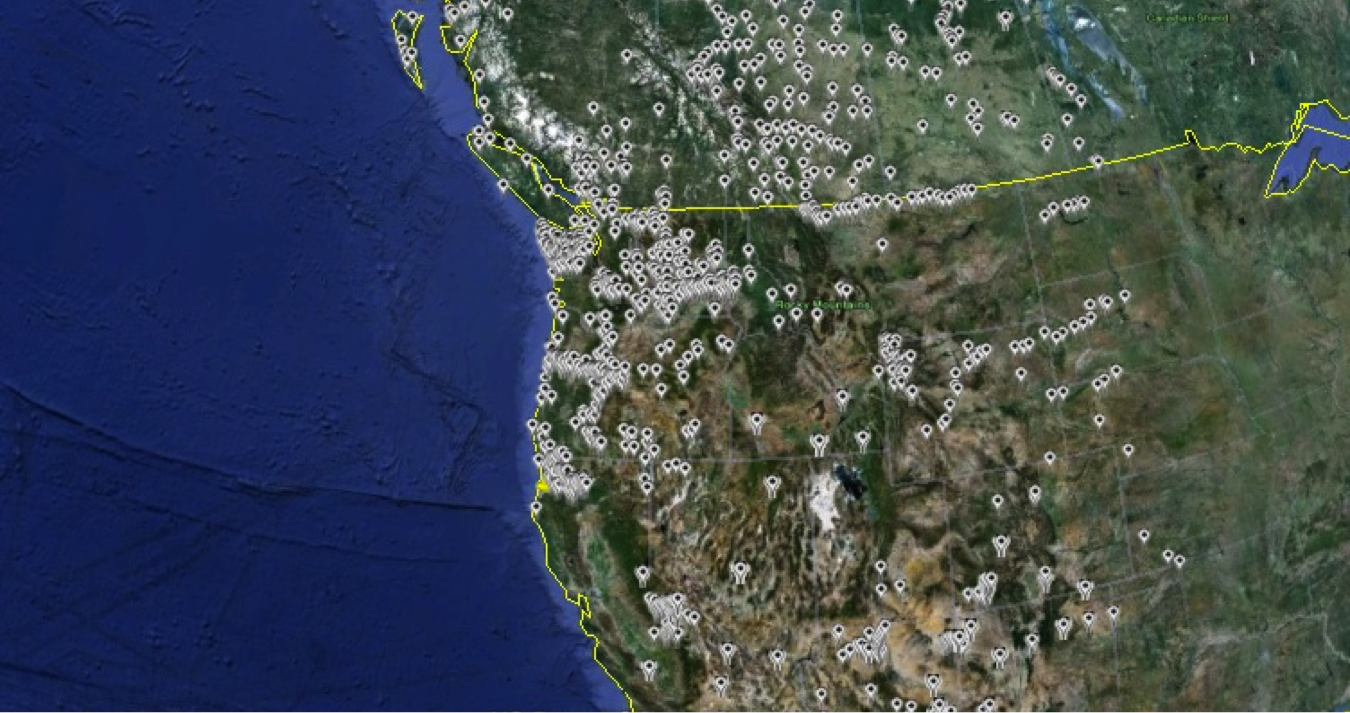
\includegraphics[width=0.8\textwidth]{./images/kmlexample.png}
% \end{center}
% \end{frame}
% 
\subsection{Raster data}
%--- Slide ----------------%
\begin{frame}{Raster data}
\begin{itemize}
  \item Area divided into regular cells or pixels with associated values
  \item Used extensively with environmental data (climate, soils, RS images, etc)
  \item Often large data files
	\item \textbf{raster} package
	\item Allows import and export of most widely used raster data formats
	\item Includes functions for raster algebra and analysis
	\item Can work of disk, avoiding memory limits
\end{itemize}
\end{frame}

%--- Slide ----------------%
\begin{frame}[fragile]{Raster data}
\begin{knitrout}\scriptsize
\definecolor{shadecolor}{rgb}{0.969, 0.969, 0.969}\color{fgcolor}\begin{kframe}
\begin{alltt}
\hlkwd{library}\hlstd{(raster)}
\hlstd{r} \hlkwb{=} \hlkwd{raster}\hlstd{(}\hlstr{"air.mon.ltm.nc"}\hlstd{,} \hlkwc{varname}\hlstd{=}\hlstr{"air"}\hlstd{)}
\hlstd{r}
\end{alltt}
\begin{verbatim}
## class      : RasterLayer 
## band       : 1  (of  12  bands)
## dimensions : 73, 144, 10512  (nrow, ncol, ncell)
## resolution : 2.5, 2.5  (x, y)
## extent     : -1.25, 358.75, -91.25, 91.25  (xmin, xmax, ymin, ymax)
## crs        : NA 
## source     : /Users/u0784726/Dropbox/DB Docs/Classes/GEOG5680/Modules/12 Spatial data in R/air.mon.ltm.nc 
## names      : Monthly.Long.Term.Mean.Air.Temperature.at.sigma.level.0.995 
## z-value    : 0000-12-30 
## zvar       : air
\end{verbatim}
\end{kframe}
\end{knitrout}
\end{frame}

%--- Slide ----------------%
\begin{frame}[fragile]{Raster data}

\begin{knitrout}\scriptsize
\definecolor{shadecolor}{rgb}{0.969, 0.969, 0.969}\color{fgcolor}
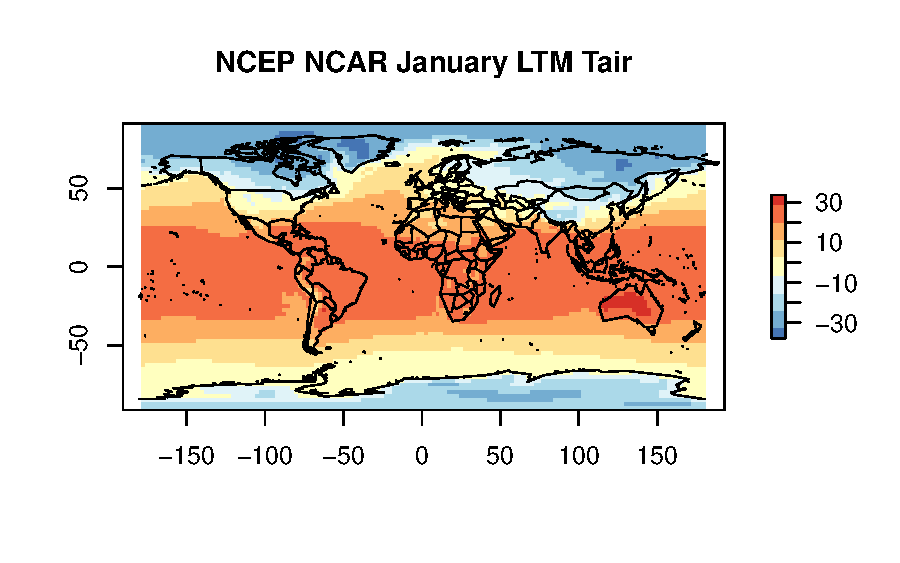
\includegraphics[width=\maxwidth]{figure/unnamed-chunk-6-1} 

\end{knitrout}
\end{frame}

% %--- Slide ----------------%
% \begin{frame}[fragile]{Visualizing spatial data}
% \begin{columns}
% 	\begin{column}{0.5\textwidth}
% 		\begin{itemize}
% 			\item Extraction by regions or shapefiles
% 			\item Summary statistics, correlations
% 			\item Raster algebra, spatial statistics
% 			\item Multi-dimensional `stacks'
% 			\item Improved visualization with \textbf{rasterVis}
% 		\end{itemize}
% 	\end{column}
% 	\begin{column}{0.5\textwidth}
% <<echo=FALSE, message=FALSE, cache=TRUE>>=
% library(raster)
% library(RColorBrewer)
% myext = extent(c(-130,-60,25,50))
% for (i in 1:12) {
%   r = rotate(raster("air.mon.ltm.nc", varname="air", band=i))
%   r = crop(r, myext)
%   if (i == 1) {
%     r.stk = stack(r)
%   } else {
%     r.stk = stack(r.stk, r)
%   }
% }
% 
% #plot(r.stk, main=paste("NCAR NCEP", month.abb), zlim=c(-20,30))
% library(rasterVis)
% us48 = readShapeSpatial("states_21basic/states.shp")
% levelplot(r.stk, names.attr=month.abb, contour=TRUE,
%           par.settings=rasterTheme(region=rev(brewer.pal(9, 'PuOr')))) +
%   layer(sp.polygons(us48))
% @
% 	\end{column}
% \end{columns}
% \end{frame}
% 
% %--- Slide ----------------%
% \begin{frame}{Next Class}
% \begin{itemize}
%   \item Lab: Spatial data in R
%   \item 0502: Web applications with R and Shiny
% \end{itemize}
% \end{frame}
% 
\end{document}
